\documentclass{template/openetcs_article}
% Use the option "nocc" if the document is not licensed under Creative Commons
%\documentclass[nocc]{template/openetcs_article}
\usepackage{lipsum,url}
\usepackage{hyperref}
\graphicspath{{./template/}{.}{./images/}}
\begin{document}
\frontmatter
\project{openETCS}

%Please do not change anything above this line
%============================
% The document metadata is defined below

%assign a report number here
\reportnum{OETCS/WP6/PG01}

%define your workpackage here
\wp{Work-Package 6: ``Dissemination \& Exploitation''}

%set a title here
\title{openETCS Publishing Guideline}

%set a subtitle here
\subtitle{ }

%set the date of the report here
\date{July 2013}

%define a list of authors and their affiliation here

\author{Stefan Rieger}

\affiliation{TWT GmbH\\
Science \& Innovation\\
Bernhäuser Straße 40-42\\
D-73765 Neuhausen\\
Germany
}

% define the coverart
\coverart[width=350pt]{openETCS_EUPL}

%define the type of report
\reporttype{Guideline}


\begin{abstract}
 All publications in the context of the openETCS project should adhere to this publishing guideline.
\end{abstract}

%=============================
%Do not change the next three lines
\maketitle
%\tableofcontents
%\listoffiguresandtables
%\newpage
%=============================

% The actual document starts below this line
%=============================

\section*{Publishing Guideline}

\begin{figure}
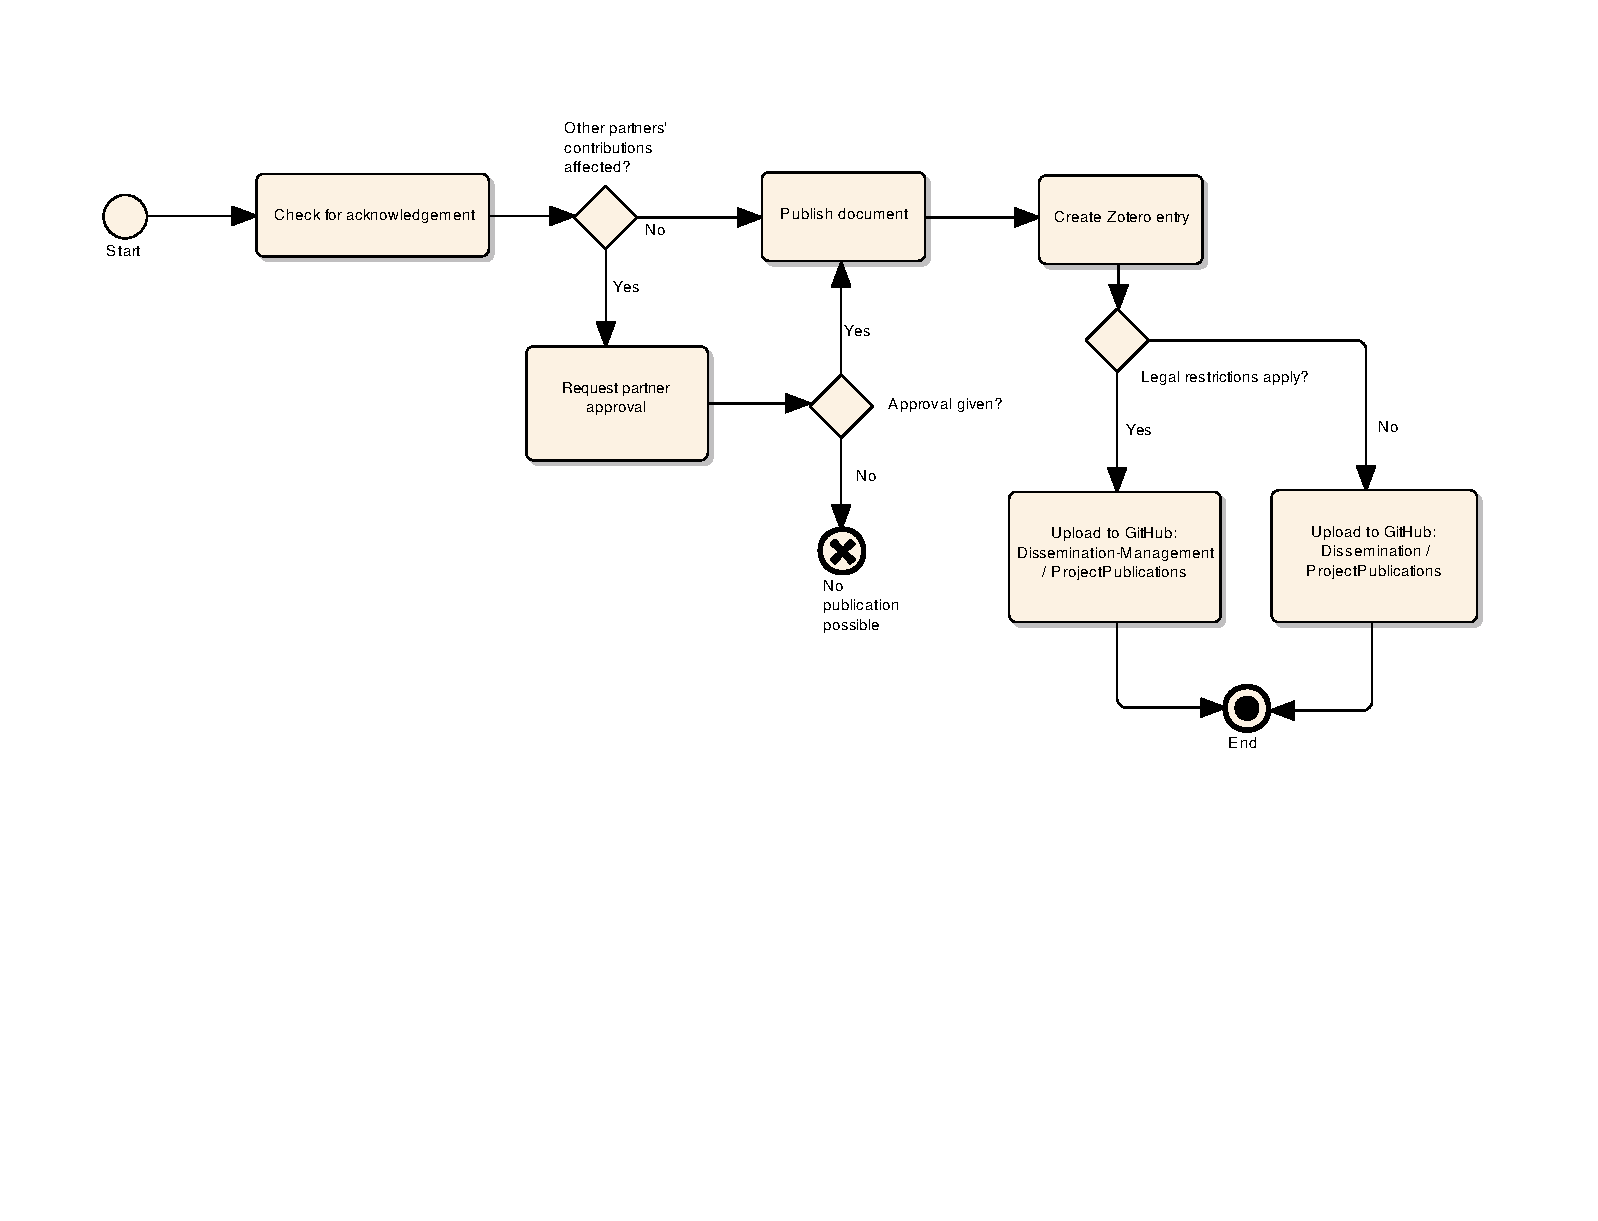
\includegraphics[trim=1.5cm 7cm 2cm 0,clip,width=\textwidth]{figs/publication_process_bpmn}
\caption{The publishing process as BPMN diagram}
\label{fig:process}
\end{figure}

When publishing in the context of the openETCS project authors shall adhere to this guideline. Figure~\ref{fig:process} depicts the steps as graphical BPMN process. The individual steps are described in detail in the following.

\begin{enumerate}
  \item  It must be ensured that the \emph{project}, the \emph{funding authority} and the \emph{grant number} is mentioned in the paper/presentation. The following acknowledgements can be used:
  \begin{description}
    \item[Germany] This work was funded by the German Federal Ministry of Education and Research (Grant No. 01IS12021) in the context of the ITEA2 project openETCS.
    \item[Belgium/Brussels region] This work was funded by the Région de Bruxelles-Capitale / Brussels Hoofdstedelijk Gewest (Grant No. RBC/12 R 11) in the context of the ITEA2 project openETCS.
    \item[Belgium/Walloon region] This work was funded by the Walloon Region (DG06) (Grant No. 6921) in the context of the ITEA2 project openETCS.
    \item[France] This work was funded by the “Direction Générale de la compétitivité, de l’industrie et des services” (DGCIS)  (Grant No. 112930309) in the context of the ITEA2 project openETCS.
    \item[to be completed] Spain still missing
  \end{description}

\item Publications potentially affecting project contributions of other partners require explicit approval. A request for approval shall be accompanied with a reasonable deadline (e.g., two weeks). Please consider a joint publication with the involved partners.

\item An entry with the details of the publication should be added to the Zotero group \emph{openETCS Publications} by using the Zotero tool or the website \href{http://www.zotero.org}{zotero.org}. A how-to regarding the use of Zotero in openETCS is \href{https://github.com/openETCS/Dissemination/wiki/Management-of-Publications-and-References-with-Zotero}{provided here}. A link to an official and public webpage where the publication can be obtained/purchased should be included.

\item The final document should be uploaded to GitHub to one of the following directories:
  \begin{itemize}
    \item To \href{https://github.com/openETCS/dissemination-management/tree/master/ProjectPublications}{Dissemination-Management/ProjectPublications} if legal restrictions apply for publication.
    \item To \href{https://github.com/openETCS/Dissemination/tree/master/ProjectPublications}{Dissemination/ProjectPublications} if it can be published freely under the openETCS Open License.
  \end{itemize}
\end{enumerate}




%\begin{thebibliography}{9}

%\bibitem{lamport94}
%  Leslie Lamport,
%  \emph{\LaTeX: A Document Preparation System}.
%  Addison Wesley, Massachusetts,
%  2nd Edition,
%  1994.

%\end{thebibliography}

%===================================================
%Do NOT change anything below this line

\end{document}
